\let\negmedspace\undefined
\let\negthickspace\undefined
\documentclass[journal,12pt,onecolumn]{IEEEtran}
\usepackage{cite}
\usepackage{amsmath,amssymb,amsfonts,amsthm}
\usepackage{algorithmic}
\usepackage{graphicx}
\graphicspath{{./figs/}}
\usepackage{textcomp}
\usepackage{xcolor}
\usepackage{txfonts}
\usepackage{listings}
\usepackage{enumitem}
\usepackage{mathtools}
\usepackage{gensymb}
\usepackage{comment}
\usepackage{caption}
\usepackage[breaklinks=true]{hyperref}
\usepackage{tkz-euclide} 
\usepackage{listings}
\usepackage{gvv}                                        
%\def\inputGnumericTable{}                                 
\usepackage[latin1]{inputenc}     
\usepackage{xparse}
\usepackage{color}                                            
\usepackage{array}                                            
\usepackage{longtable}                                       
\usepackage{calc}                                             
\usepackage{multirow}
\usepackage{multicol}
\usepackage{hhline}                                           
\usepackage{ifthen}                                           
\usepackage{lscape}
\usepackage{tabularx}
\usepackage{array}
\usepackage{float}
\newtheorem{theorem}{Theorem}[section]
\newtheorem{problem}{Problem}
\newtheorem{proposition}{Proposition}[section]
\newtheorem{lemma}{Lemma}[section]
\newtheorem{corollary}[theorem]{Corollary}
\newtheorem{example}{Example}[section]
\newtheorem{definition}[problem]{Definition}
\newcommand{\BEQA}{\begin{eqnarray}}
\newcommand{\EEQA}{\end{eqnarray}}
\newcommand{\define}{\stackrel{\triangle}{=}}
\theoremstyle{remark}
\newtheorem{rem}{Remark}

\begin{document}
\title{
ASSIGNMENT 6: gate 2018 \\
    BT : BIOTECHNOLOGY }
\author{AI25BTECH11035 - Sujal Rajani }
\maketitle
\renewcommand{\thefigure}{\theenumi}
\renewcommand{\thetable}{\theenumi}

    

\textbf{Q.1 -- Q.5 carry one mark each.}
\begin{enumerate}
   
    \item ``When she fell down the \underline{\hspace{2cm}}, she received many \underline{\hspace{2cm}} but little help.''\\
    The words that best fill the blanks in the above sentence are
    \begin{multicols}{2}
    \begin{enumerate}
        \item stairs, stares
        \item stairs, stairs
        \item stares, stairs
        \item stares, stares
    \end{enumerate}
\end{multicols}

    \item ``In spite of being warned repeatedly, he failed to correct his \underline{\hspace{2cm}} behaviour.''\\
    The word that best fills the blank in the above sentence is
    \begin{multicols}{4}
        
    
    \begin{enumerate}
        \item rational
        \item reasonable
        \item errant
        \item good
    \end{enumerate}
\end{multicols}
    \item For $0 \leq x \leq 2\pi$, $\sin x$ and $\cos x$ are both decreasing functions in the interval \underline{\hspace{2cm}}
    \begin{multicols}{4}
    \begin{enumerate}
        \item $(0, \frac{\pi}{2})$
        \item $(\frac{\pi}{2}, \pi)$
        \item $(\pi, \frac{3\pi}{2})$
        \item $(\frac{3\pi}{2}, 2\pi)$
    \end{enumerate}
\end{multicols}
    \item The area of an equilateral triangle is $\sqrt{3}$. What is the perimeter of the triangle?
    \begin{multicols}{4}
        
    
    \begin{enumerate}
        \item 2
        \item 4
        \item 6
        \item 8
    \end{enumerate}
\end{multicols}
    \item Arrange the following three-dimensional objects in the descending order of their volumes:\\
    (i) A cuboid with dimensions $10$ cm, $8$ cm and $6$ cm\\
    (ii) A cube of side $8$ cm\\
    (iii) A cylinder with base radius $7$ cm and height $7$ cm\\
    (iv) A sphere of radius $7$ cm

    \begin{enumerate}
        \item (i), (ii), (iii), (iv)
        \item (ii), (i), (iv), (iii)
        \item (iii), (ii), (i), (iv)
        \item (iv), (iii), (ii), (i)
    \end{enumerate}
    \textbf{Q6-Q10 carry two marks each}
    \item An automobile travels from city A to city B and returns to city A by the same route. The speed of the vehicle during the onward and return journeys were constant at 60 km/h and 90 km/h, respectively. What is the average speed in km/h for the entire journey?
    \begin{enumerate}
\begin{multicols}{4}
\item 72
\item 73
\item 74
\item 75
\end{multicols}
 \end{enumerate}
    \item A set of $4$ parallel lines intersect with another set of $5$ parallel lines. How many parallelograms are formed?
    \begin{multicols}{4}
    \begin{enumerate}
        \item 20
        \item 48
        \item 60
        \item 72
    \end{enumerate}
    \end{multicols}

    \item To pass a test, a candidate needs to answer at least $2$ out of $3$ questions correctly. A total of $6,30,000$ candidates appeared for the test. Question A was correctly answered by $3,30,000$ candidates. Question B was answered correctly by $2,50,000$ candidates. Question C was answered correctly by $2,60,000$ candidates. Both questions A and B were answered correctly by $1,00,000$ candidates. Both questions B and C were answered correctly by $90,000$ candidates. Both questions A and C were answered correctly by $80,000$ candidates. If the number of students answering all questions correctly is the same as the number answering none, how many candidates failed to clear the test?
    \begin{multicols}{4}
    \begin{enumerate}
        \item 30,000
        \item 2,70,000
        \item 3,90,000
        \item 4,20,000
    \end{enumerate}
    \end{multicols}

    \item If $x^2 + x - 1 = 0$, what is the value of $x^4 + \frac{1}{x^4}$?
    \begin{multicols}{4}
    \begin{enumerate}
        \item 1
        \item 5
        \item 7
        \item 9
    \end{enumerate}
    \end{multicols}

    \item In a detailed study of annual crow births in India, it was found that there was relatively no growth during the period $2002$ to $2004$ and a sudden spike from $2004$ to $2005$. In another unrelated study, it was found that the revenue from cracker sales in India, which remained fairly flat from $2002$ to $2004$, saw a sudden spike in $2005$ before declining again in $2006$. The solid line in the graph below refers to annual sale of crackers and the dashed line refers to the annual crow births in India. Choose the most appropriate inference from the above data.

   \begin{figure}[H]
    \centering
    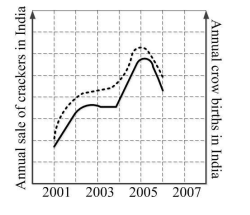
\includegraphics[width = 0.5\columnwidth]{fig/Q10.png}
    \caption*{}
    \label{fig:Q10}
\end{figure}
    
    \begin{enumerate}
        \item There is a strong correlation between crow birth and cracker sales.
        \item Cracker usage increases crow birth rate.
        \item If cracker sale declines, crow birth will decline.
        \item Increased birth rate of crows will cause an increase in the sale of crackers.
    \end{enumerate}
    
\end{enumerate}
{\textbf{END OF THE QUESTION PAPER}}
\newpage
    \section*{Q.1 -- Q.25 carry one mark each.}

\begin{enumerate}
    \item Consider an unfair coin. The probability of getting heads is $0.6$. If you toss this coin twice, what is the probability that the first or the second toss is heads?
    \begin{multicols}{4}
    \begin{enumerate}
        \item 0.56
        \item 0.64
        \item 0.84
        \item 0.96
    \end{enumerate}
    \end{multicols}
    
    \item If serum is removed from the growth medium of human embryonic kidney cell line (HEK), then the cells will
    
    \begin{enumerate}
        \item proliferate faster
        \item proliferate normally
        \item undergo cell cycle arrest
        \item undergo immediate apoptosis
    \end{enumerate}
   

    \item The repeat sequence of telomere in humans is
    \begin{multicols}{2}
    \begin{enumerate}
        \item 5'-TATAAT-3'
        \item 5'-TTAGGG-3'
        \item 5'-GGGCCC-3'
        \item 5'-AAAAAA-3'
    \end{enumerate}
    \end{multicols}

    \item If a segment of a sense strand of DNA is 5'-ATGGACCAGA-3', then the resulting RNA sequence after transcription is
    \begin{multicols}{2}
    \begin{enumerate}
        \item 5'-AGACCAGGTA-3'
        \item 5'-UCUCGGUCCAU-3'
        \item 5'-UACCGUGCUC-3'
        \item 5'-AUGGACCAGA-3'
    \end{enumerate}
    \end{multicols}
    
    \item Which one of the following is an example of a neurotoxin?
    
    \begin{enumerate}
        \item Cholera toxin
        \item Streptolysin-O
        \item Botulinum toxin
        \item Diphtheria toxin
    \end{enumerate}
    

    \item Which of the following components constitute a molecular mechanics force field?\\
    P. Bond stretching\\
    Q. Bond angle bending\\
    R. Torsional bond rotation\\
    S. Non-bonded interactions
   
    \begin{enumerate}
        \item P and Q only
        \item P, Q and R only
        \item P, Q and S only
        \item P, Q, R and S
    \end{enumerate}
    

    \item Which one of the following BLAST search programs is used to identify homologs of a genomic DNA query in a protein sequence database?
    \begin{multicols}{4}
    \begin{enumerate}
        \item blastp
        \item blastn
        \item blastx
        \item tblastn
    \end{enumerate}
    \end{multicols}
 \item A mixture contains three similarly sized peptides P, Q and R. The peptide P is positively charged, Q is weakly negative and R is strongly negative. If this mixture is passed through an ion-exchange chromatography column containing an anionic resin, their order of elution will be
    \begin{multicols}{2}
    \begin{enumerate}
        \item P, Q, R
        \item R, Q, P
        \item Q, R, P
        \item P, Q and R elute together
    \end{enumerate}
    \end{multicols}

    \item Which one of the following is \textbf{INCORRECT} about protein structures?
    
    \begin{enumerate}
        \item A protein fold is stabilized by favorable non-covalent interactions
        \item All parts of a fold can be classified as helices, strands or turns
        \item Two non-covalent atoms cannot be closer than the sum of their van der Waals radii
        \item The peptide bond is nearly planar
    \end{enumerate}
    

    \item Which one of the following metabolic processes in mammalian cells does \textbf{NOT} occur in the mitochondria?
    \begin{multicols}{2}
    \begin{enumerate}
        \item Citric acid cycle
        \item Oxidative phosphorylation
        \item Fatty acid $\beta$-oxidation
        \item Glycolysis
    \end{enumerate}
    \end{multicols}
    
    \item Which one of the following is \textbf{NOT} a principal component of innate immunity?
    
    \begin{enumerate}
        \item Mucosal epithelia
        \item Dendritic cells
        \item Complement system
        \item Memory B-cells
    \end{enumerate}

    \item Which of the following technique(s) can be used to study conformational changes in myoglobin?\\
        P. Mass spectrometry\\
        Q. Fluorescence spectroscopy\\
        R. Circular dichroism spectroscopy\\
        S. Light microscopy
    \begin{multicols}{4}
    \begin{enumerate}
        \item P only
        \item P and S only
        \item Q and R only
        \item S only
    \end{enumerate}
    \end{multicols}

    \item Which one of the following bioreactor configurations is the basis for a trickling biological filter?
    \begin{multicols}{2}
    \begin{enumerate}
        \item Stirred tank
        \item Packed bed
        \item Air lift
        \item Fluidized bed
    \end{enumerate}
    \end{multicols}
\item Cell type A secretes molecule X into the culture medium. Cell type B in the same culture responds to the molecule X by expressing protein Y. Which one of the following modes of signaling represents the interaction between A and B?
    \begin{multicols}{2}
    \begin{enumerate}
        \item Autocrine
        \item Juxtacrine
        \item Paracrine
        \item Intracrine
    \end{enumerate}
    \end{multicols}

    \item Which one of the following statements is true for actin?
    
    \begin{enumerate}
        \item Actin filament is structurally polarized and the two ends are not identical
        \item \textit{De novo} actin polymerization is a single-step process
        \item The pointed end of the actin filaments is the fast growing end
        \item Actin forms spindle fibers during mitosis
    \end{enumerate}
    

    \item Standard error is
    
    \begin{enumerate}
        \item the probability of a type I error in a statistical test
        \item the error in estimating a sample standard deviation
        \item the standard deviation of a variable that follows standard normal distribution
        \item the standard deviation of distribution of sample means
    \end{enumerate}
    
    \item Which one of the following techniques is used to monitor RNA transcripts, both temporally and spatially?
   
    \begin{enumerate}
        \item Northern blotting
        \item \textit{In situ} hybridization
        \item Southern blotting
        \item Western blotting
    \end{enumerate}
    

    \item Identify the character based method(s) used for the construction of a phylogenetic tree.\\
    P. Maximum parsimony\\
    Q. Neighbor joining\\
    R. Maximum likelihood\\
    S. Bootstrapping
    \begin{multicols}{2}
    \begin{enumerate}
        \item Q only
        \item P and R only
        \item Q and S only
        \item S only
    \end{enumerate}
    \end{multicols}

    \item Which one of the following is the solution for $\cos^2x + 2\cos x + 1 = 0$, for values of $x$ in the range of $0^\circ < x < 360^\circ$?
    \begin{multicols}{4}
    \begin{enumerate}
        \item $45^\circ$
        \item $90^\circ$
        \item $180^\circ$
        \item $270^\circ$
    \end{enumerate}
    \end{multicols}

    \item Which one of the following plant secondary metabolites is a natural insecticide?
    \begin{multicols}{4}
    \begin{enumerate}
        \item Digitoxin
        \item Pyrethrin
        \item Salicylic acid
        \item Avenacin A-1
    \end{enumerate}
    \end{multicols}
    \item The determinant of the matrix
    $
        \myvec{
            4 & -6 \\
            -3 & 2
        }
    $
    is \underline{\hspace{2cm}}
    
    \item The variable $z$ has a standard normal distribution. If $P(0 \leq z \leq 1) = 0.34$, then $P(z^2 > 1)$ is equal to (up to two decimal places) \underline{\hspace{2cm}}
    
    \item The absorbance of a solution of tryptophan measured at $280\,\mathrm{nm}$ in a cuvette of $2.0\,\mathrm{cm}$ path length is $0.56$ at $pH\,7$. The molar extinction coefficient $(\varepsilon)$ for tryptophan at $280\,\mathrm{nm}$ is $5600\,\mathrm{M}^{-1}\mathrm{cm}^{-1}$ at $pH\,7$. The concentration of tryptophan (in $\mu$M) in the solution is \underline{\hspace{2cm}}
    
    \item A single stem cell undergoes 10 asymmetric cell divisions. The number of stem cells at the end is \underline{\hspace{2cm}}
    
    \item Genomic DNA isolated from a bacterium was digested with a restriction enzyme that recognizes a $6$-base pair (bp) sequence. Assuming random distribution of bases, the average length (in bp) of the fragments generated is \underline{\hspace{2cm}}

{\textbf{Q.26 -- Q.55 carry two marks each.}}


    \item In leguminous plants, both the rhizobium genes and the plant genes influence nodulation and nitrogen fixation. Which one of the following functions is \textbf{NOT} encoded by the host plant genes?
    
    \begin{enumerate}
        \item Production of inducers that modify rhizobial cell wall
        \item Production of flavonoid inducers
        \item Establishment of contact between bacteria and legume
        \item Root hair curling
    \end{enumerate}
    

    \item Which of the following cytokines are endogenous pyrogens?\\
    P. Tumor necrosis factor-$\alpha$\\
    Q. Interleukin-1\\
    R. Transforming growth factor-$\beta$\\
    S. Interleukin-10
    
    \begin{enumerate}
        \item P and Q only
        \item P and R only
        \item R and S only
        \item Q and S only
    \end{enumerate}
    

    \item Match the classes of RNA molecules in Group I with their functions in Group II.

    \begin{tabbing}
    Group I \hspace{2cm} \= Group II \\
    P. snoRNA    \> 1. Protects germline from transposable elements \\
    Q. piRNA     \> 2. Blocks translation of selected mRNA \\
    R. miRNA     \> 3. Template for telomere elongation \\
    S. snRNA     \> 4. Modification and processing of rRNA \\
                  \> 5. Splicing of RNA transcripts
    \end{tabbing}
    \vspace{-0.8em}
    \begin{multicols}{2}
    \begin{enumerate}
        \item P-3, Q-5, R-2, S-4
        \item P-1, Q-3, R-2, S-5
        \item P-1, Q-4, R-5, S-2
        \item P-4, Q-1, R-2, S-5
    \end{enumerate}
    \end{multicols}

    \item Determine the correctness or otherwise of the following Assertion [a] and the Reason [r]\\
    \textbf{Assertion}: \textit{Ab initio} gene finding algorithms that predict protein coding genes in eukaryotic genomes are not completely accurate.\\
    \textbf{Reason}: Eukaryotic splice sites are difficult to predict.
    
    \begin{enumerate}
        \item Both [a] and [r] are false
        \item [a] is true but [r] is false
        \item Both [a] and [r] are true and [r] is the correct reason for [a]
        \item Both [a] and [r] are true but [r] is not the correct reason for [a]
    \end{enumerate}
    \item Which one of the following amino acids is catalyzed by activated macrophages to produce reactive nitrogen species?
    \begin{multicols}{2}
    \begin{enumerate}
        \item Arginine
        \item Asparagine
        \item Cysteine
        \item Histidine
    \end{enumerate}
    \end{multicols}

    \item Determine the correctness or otherwise of the following Assertion [a] and the Reason [r]\\
    Assertion: The association constant in water for the G-C base pair is three times lower than that for the A-T base pair.\\
    Reason: There are three hydrogen bonds in the G-C base pair and two in the A-T base pair.
    \begin{multicols}{2}
    \begin{enumerate}
        \item Both [a] and [r] are true and [r] is the correct reason for [a]
        \item [a] is false but [r] is true
        \item Both [a] and [r] are false
        \item Both [a] and [r] are true and [r] is not the correct reason for [a]
    \end{enumerate}
    \end{multicols}

    \item Which one of the combinations of the following statements is true about antibody structure?\\
    P. Limited proteolysis of rabbit IgG with the enzyme pepsin generates two antigen-binding regions (Fab) and an Fc fragment\\
    Q. Limited proteolysis of rabbit IgG with the enzyme papain generates a single bivalent antigen-binding region F(ab$'$)$_2$ and peptide fragments\\
    R. The Fc fragment of IgG can self-associate and crystallize into a lattice\\
    S. The F(ab$'$)$_2$ fragment of IgG is composed of both light and heavy chains
    \begin{multicols}{2}
    \begin{enumerate}
        \item P and Q only
        \item P and R only
        \item R and S only
        \item Q and S only
    \end{enumerate}
    \end{multicols}

    \item Which one of the following statements is true with regard to processing and presentation of protein antigens?
   
    \begin{enumerate}
        \item In the class II MHC pathway, protein antigens in the cytosol are processed by proteasomes
        \item In the class I MHC pathway, extracellular protein antigens are endocytosed into vesicles and processed
        \item In the class I MHC pathway, transporter associated antigen processing (TAP) protein is required for translocating processed peptides generated in the cytosol
        \item Invariant chain in endoplasmic reticulum is involved in transport of peptides and loading of class I MHC
    \end{enumerate}
   
    \item Which of the following are true about bacterial superoxide dismutase?\\
    P. Present in obligate aerobes\\
    Q. Present in facultative anaerobes\\
    R. Present in aerotolerant anaerobes\\
    S. Absent in obligate aerobes
    \begin{multicols}{2}
    \begin{enumerate}
        \item P and Q only
        \item P, Q and R only
        \item Q and S only
        \item P and S only
    \end{enumerate}
    \end{multicols}
    \item Which of the following are true with regard to anaerobic respiration in bacteria?\\
    P. The final electron acceptor is an inorganic substance other than molecular oxygen\\
    Q. The number of ATP molecules produced per glucose molecule is more than that produced in aerobic respiration\\
    R. The number of ATP molecules produced per glucose molecule is less than that produced in aerobic respiration\\
    S. Only substrate level phosphorylation is used to generate ATP
    \begin{multicols}{2}
    \begin{enumerate}
        \item P and S only
        \item Q and S only
        \item P and R only
        \item P, Q and S only
    \end{enumerate}
    \end{multicols}

    \item Shear stress versus shear rate behavior of four different types of fluids (I, II, III and IV) are shown in the figure below.
    \begin{figure}[H]
    \centering
    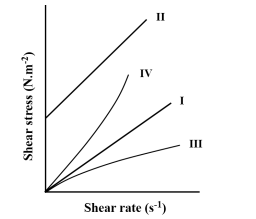
\includegraphics[width = 0.5\columnwidth]{fig/Q36.png}
    \caption*{}
    \label{fig:Q36}
\end{figure}
    Which one of the following options is correct?
    
    \begin{enumerate}
        \item I-Newtonian, II-Bingham plastic, III-Dilatant, IV-Pseudoplastic
        \item I-Pseudoplastic, II-Dilatant, III-Newtonian, IV-Bingham plastic
        \item I-Newtonian, II-Pseudoplastic, III-Bingham plastic, IV-Dilatant
        \item I-Newtonian, II-Bingham plastic, III-Pseudoplastic, IV-Dilatant
    \end{enumerate}
    
    \item An analysis of DNA-protein interactions was carried out using all DNA-protein complexes in the protein data bank (PDB). The frequency distribution of four amino acid residues, represented as P, Q, R and S, occurring in non-covalent interactions between the protein and DNA backbone is shown below.
\begin{figure}[H]
    \centering
    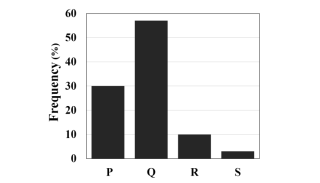
\includegraphics[width = 0.5\columnwidth]{fig/Q37.png}
    \caption*{}
    \label{fig:Q37}
\end{figure}
   
    Which one of the following is correct?
    \begin{multicols}{2}
    \begin{enumerate}
        \item P-Lys, Q-Arg, R-Gln, S-Glu
        \item P-Gln, Q-Glu, R-Lys, S-Arg
        \item P-Asn, Q-Asp, R-Arg, S-Lys
        \item P-His, Q-Glu, R-Gln, S-Lys
    \end{enumerate}
    \end{multicols}

    \item A pedigree of an inheritable disease is shown below.
\begin{figure}[H]
    \centering
    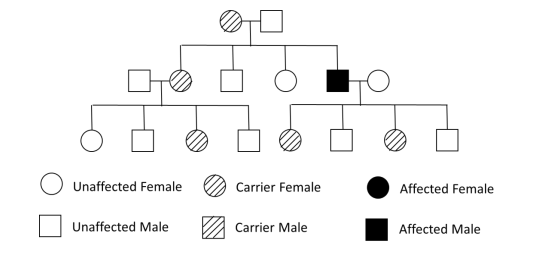
\includegraphics[width = 0.5\columnwidth]{fig/Q38.png}
    \caption*{}
    \label{fig:Q38}
\end{figure}
   
    What type of inheritance does the disease follow?
    \begin{multicols}{2}
    \begin{enumerate}
        \item Autosomal dominant
        \item X-linked dominant
        \item X-linked recessive
        \item Autosomal recessive
    \end{enumerate}
    \end{multicols}
    \item Match the industrial products mentioned in Group I with their producer organisms in Group II.

    \begin{tabbing}
    Group I \hspace{1.5cm} \= Group II \\
    P. Citric acid \> 1. \textit{Trichoderma viride} \\
    Q. Cellulase \> 2. \textit{Clostridium acetobutylicum} \\
    R. Vitamin B$_{12}$ \> 3. \textit{Aspergillus niger} \\
    S. Butanol \> 4. \textit{Propionibacterium freudenreichii}
    \end{tabbing}

    \begin{multicols}{2}
    \begin{enumerate}
        \item P-4, Q-3, R-1, S-2
        \item P-3, Q-1, R-2, S-4
        \item P-2, Q-1, R-4, S-3
        \item P-3, Q-1, R-4, S-2
    \end{enumerate}
    \end{multicols}

    \item 5' capping of mRNA transcripts in eukaryotes involves the following events:\\
    P. Addition of GMP on the 5' end\\
    Q. Removal of $\gamma$-phosphate of the triphosphate on first base at the 5' end\\
    R. 5'-5' linkage between GMP and the first base at 5' end\\
    S. Addition of methyl group to N7 position of guanine

    Which one of the following is the correct sequence of events?
    \begin{multicols}{2}
    \begin{enumerate}
        \item P, Q, R, S
        \item P, R, Q, S
        \item Q, P, R, S
        \item Q, P, S, R
    \end{enumerate}
    \end{multicols}

    \item Calculate the following integral (up to two decimal places):
    \begin{align*}
        \int_0^1 (x+3)(x+1) dx = \underline{\hspace{2cm}}
    \end{align*}
    
    \item The probability distribution for a discrete random variable $X$ is given below.
   \begin{figure}[H]
    \centering
    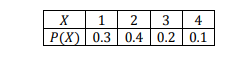
\includegraphics[width = 0.4\columnwidth]{fig/Q42.png}
    \caption*{}
    \label{fig:Q42}
\end{figure}
   
    The expectation value of $X$ is (up to one decimal place) \underline{\hspace{2cm}}

    \item If $1 + r + r^2 + r^3 + \dots \infty = 1.5$,
    then, $1 + 2r + 3r^2 + 4r^3 + \dots \infty = $ (up to two decimal places) \underline{\hspace{2cm}}
    \item Moist heat sterilization of spores at $121^\circ$C follows first order kinetics as per the expression:
    \begin{align*}
        \frac{dN}{dt} = -k_d N
    \end{align*}
        
    
    where $N$ is the number of viable spores, $t$ is the time, $k_d$ is the rate constant and $\frac{dN}{dt}$ is the rate of change of viable spores.\\
    If $k_d$ value is $1.0\ \text{min}^{-1}$, the time (in minutes) required to reduce the number of viable spores from an initial value of $10^{10}$ to a final value of $1$ is (up to two decimal places) \underline{\hspace{2cm}}
    
    \item An aqueous solution containing $6.8\ \text{mg/L}$ of an antibiotic is extracted with amyl acetate. If the partition coefficient of the antibiotic is $170$ and the ratio of water to solvent is $85$, then the extraction factor is \underline{\hspace{2cm}}
    
    \item A microbial strain is cultured in a $100$ L stirred fermenter for secondary metabolite production. If the specific rate of oxygen uptake is $0.4$ h$^{-1}$ and the oxygen solubility in the broth is $8$ mg/L, then the volumetric mass transfer coefficient ($K_L a$) (in s$^{-1}$) of oxygen required to achieve a maximum cell concentration of $12$ g/L is (up to two decimal places) \underline{\hspace{2cm}}
    
    \item In a chemostat, the feed flow rate and culture volume are $100$ ml/h and $1.0$ L, respectively. With glucose as substrate, the values of $\mu_{max}$ and $K_s$ are $0.2$ h$^{-1}$ and $1$ g/L, respectively. For a glucose concentration of $10$ g/L in the feed, the effluent substrate concentration (in g/L) is \underline{\hspace{2cm}}
    
    \item Mammalian cells in active growth phase were seeded at a density of $1 \times 10^5$ cells/ml. After $72$ hours, $1 \times 10^6$ cells/ml were obtained. The population doubling time of the cells in hours is (up to two decimal places) \underline{\hspace{2cm}}
    
    \item Yeast converts glucose to ethanol and carbon dioxide by glycolysis as per the following reaction:
    \begin{align*}
        {C_6H_{12}O_6} \rightarrow 2{C_2H_5OH} + 2{CO_2}
     \end{align*}
    Assuming complete conversion, the amount of ethanol produced (in g) from $200$ g of glucose is (up to two decimal places) \underline{\hspace{2cm}}
    \item At the end of a batch culture, glucose solution is added at a flow rate of $200$ ml/h. If the culture volume after $2$ h of glucose addition is $1000$ ml, the initial culture volume (in ml) is \underline{\hspace{2cm}}
    
    \item Consider the following alignment of two DNA sequences:
    \begin{verbatim}
    AGTAAC
    AA--AC
    \end{verbatim}
    Assuming an affine gap scoring scheme of an identity matrix for substitution, a gap initiation penalty of $1$ and a gap extension penalty of $0.1$, the score of the alignment is (up to one decimal place) \underline{\hspace{2cm}}
    
    \item First order deactivation rate constants for soluble and immobilized amyloglucosidase enzyme are $0.03$ min$^{-1}$ and $0.005$ min$^{-1}$, respectively. The ratio of half-life of the immobilized enzyme to that of the soluble enzyme is (rounded off to the nearest integer) \underline{\hspace{2cm}}
    
    \item Consider a simple uni-substrate enzyme that follows Michaelis-Menten kinetics. When the enzyme catalyzed reaction was carried out in the presence of $10$ nM concentration of an inhibitor, there was no change in the maximal velocity. However, the slope of the Lineweaver-Burk plot increased $3$-fold. The dissociation constant for the enzyme-inhibitor complex (in nM) is \underline{\hspace{2cm}}

    \item The product of complete digestion of the plasmid shown below with EcoRI and HaeIII was purified and used as a template in a reaction containing Klenow fragment of DNA polymerase, dNTPs and [$\alpha$-$^{32}$P]-dATP in a suitable reaction buffer. The product thus obtained was purified and subjected to gel electrophoresis followed by autoradiography.
    \begin{figure}[H]
    \centering
    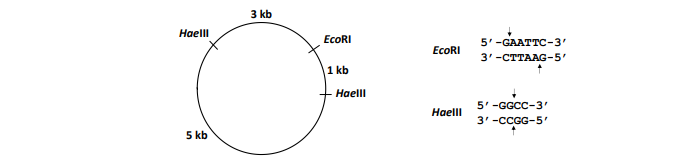
\includegraphics[width = 1.5\columnwidth]{fig/Q54.png}
    \caption*{}
    \label{fig:Q54}
\end{figure}
    The number of bands that will appear on the X-ray film is \underline{\hspace{2cm}} 
   \item A rod shaped bacterium has a length of 2 $\mu m$ m, diameter of 1 $\mu m$and density the same as that 
of water. If proteins constitute 15 of the cell mass and the average protein has a mass of   50 kDa, the number of proteins in the cell is\underline{\hspace{2cm}}
(1 Da = 1.6 x 10-24g)
\end{enumerate}
\end{document}
